\section{Design Documents}
\section{Testing Results}

\section{Evaluation Data}
\subsection{Twitter Analytics Data}


\begin{figure}
\centering
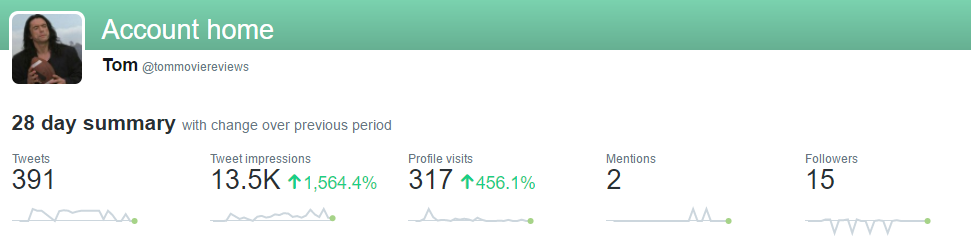
\includegraphics[width=0.7\linewidth]{figures/twitter_analytics/28daysummary}
\caption{28 Day Summary of Twitter Bot Analytics}
\label{fig:28daysummary}
\end{figure}
\begin{figure}
\centering
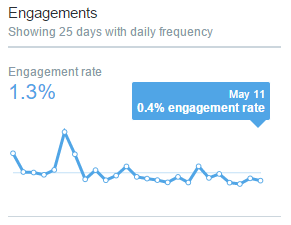
\includegraphics[width=0.7\linewidth]{figures/twitter_analytics/engagements}
\caption{Total number of 'engagements' with twitter bot over active period}
\label{fig:engagements}
\end{figure}
\begin{figure}
\centering
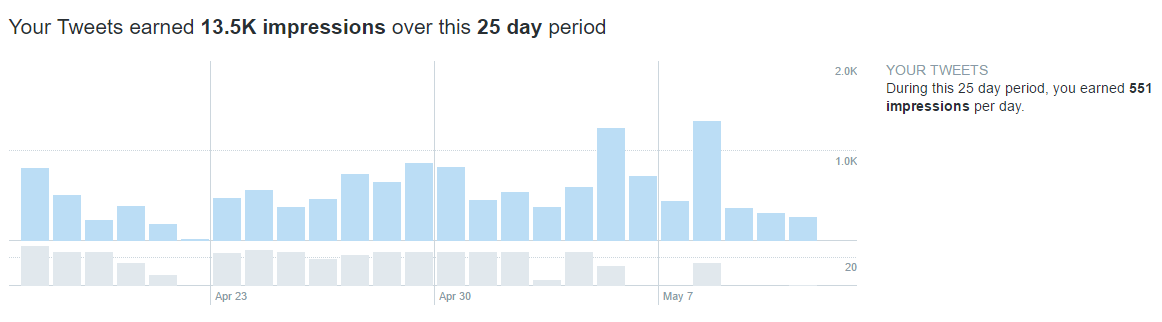
\includegraphics[width=0.7\linewidth]{figures/twitter_analytics/impressions}
\caption{Total number of 'impressions' made by twitter bot over active period}
\label{fig:impressions}
\end{figure}
\begin{figure}
\centering
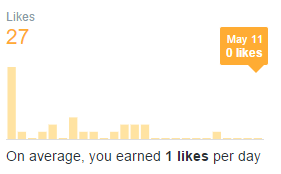
\includegraphics[width=0.7\linewidth]{figures/twitter_analytics/likes}
\caption{Likes obtained over active period}
\label{fig:likes}
\end{figure}
\begin{figure}
\centering
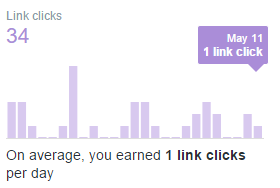
\includegraphics[width=0.7\linewidth]{figures/twitter_analytics/linkclicks}
\caption{Links clicked over active period}
\label{fig:linkclicks}
\end{figure}
\begin{figure}
\centering
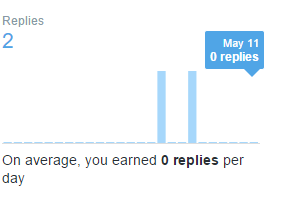
\includegraphics[width=0.7\linewidth]{figures/twitter_analytics/replies}
\caption{Replies to posts made by bot over active period}
\label{fig:replies}
\end{figure}
\begin{figure}
\centering
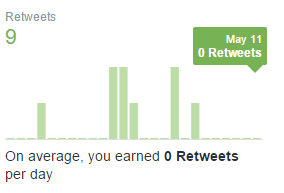
\includegraphics[width=0.7\linewidth]{figures/twitter_analytics/retweets}
\caption{Retweets of posts made by bot over active period}
\label{fig:retweets}
\end{figure}



\subsection{Google Analytics Data}
\begin{figure}
\centering
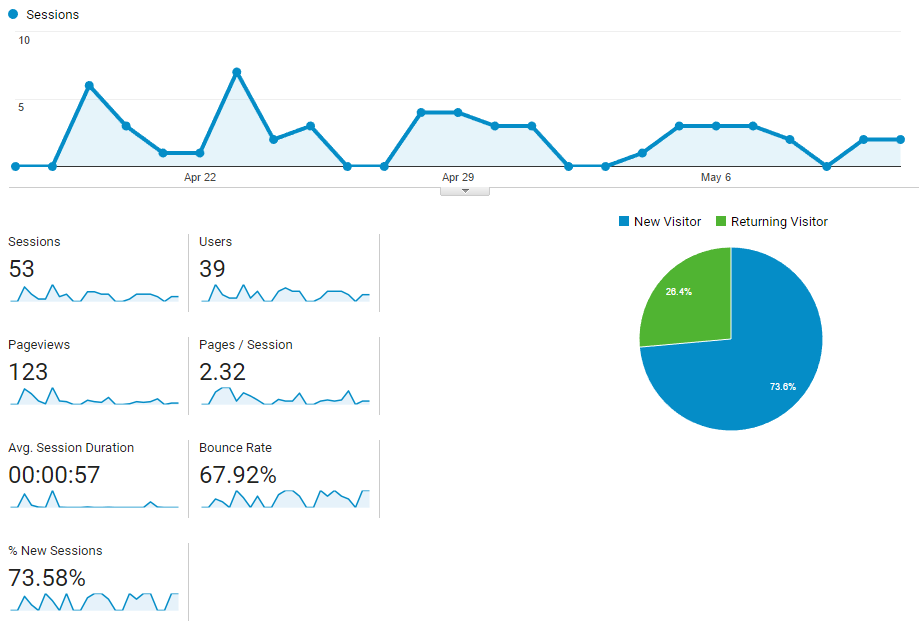
\includegraphics[width=0.7\linewidth]{figures/google_analytics/uniqueSessions}
\caption{Google Analytics Screenshot showing unique sessions over test period}
\label{fig:uniquesessions}
\end{figure}
\begin{figure}
\centering
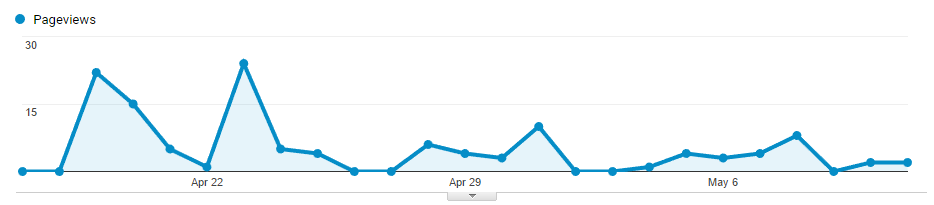
\includegraphics[width=0.7\linewidth]{figures/google_analytics/pageviews}
\caption{Google Analytics Screenshot showing pageviews over test period}
\label{fig:pageviews}
\end{figure}
\begin{figure}
\centering
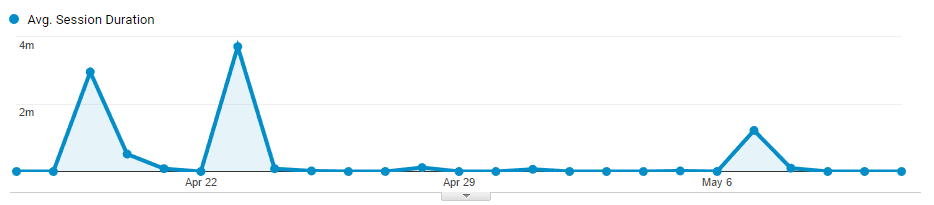
\includegraphics[width=0.7\linewidth]{figures/google_analytics/sessionDuration}
\caption{Google Analytics Screenshot showing average session duration over test period}
\label{fig:sessionduration}
\end{figure}

\subsection{Turing-Like Test Results}


\includepdf[pages={1-},scale=1]{"figures/turinglike_results/Review Feedback - reviewExcerpt (1)"}      


\section{Preliminary Project Report}


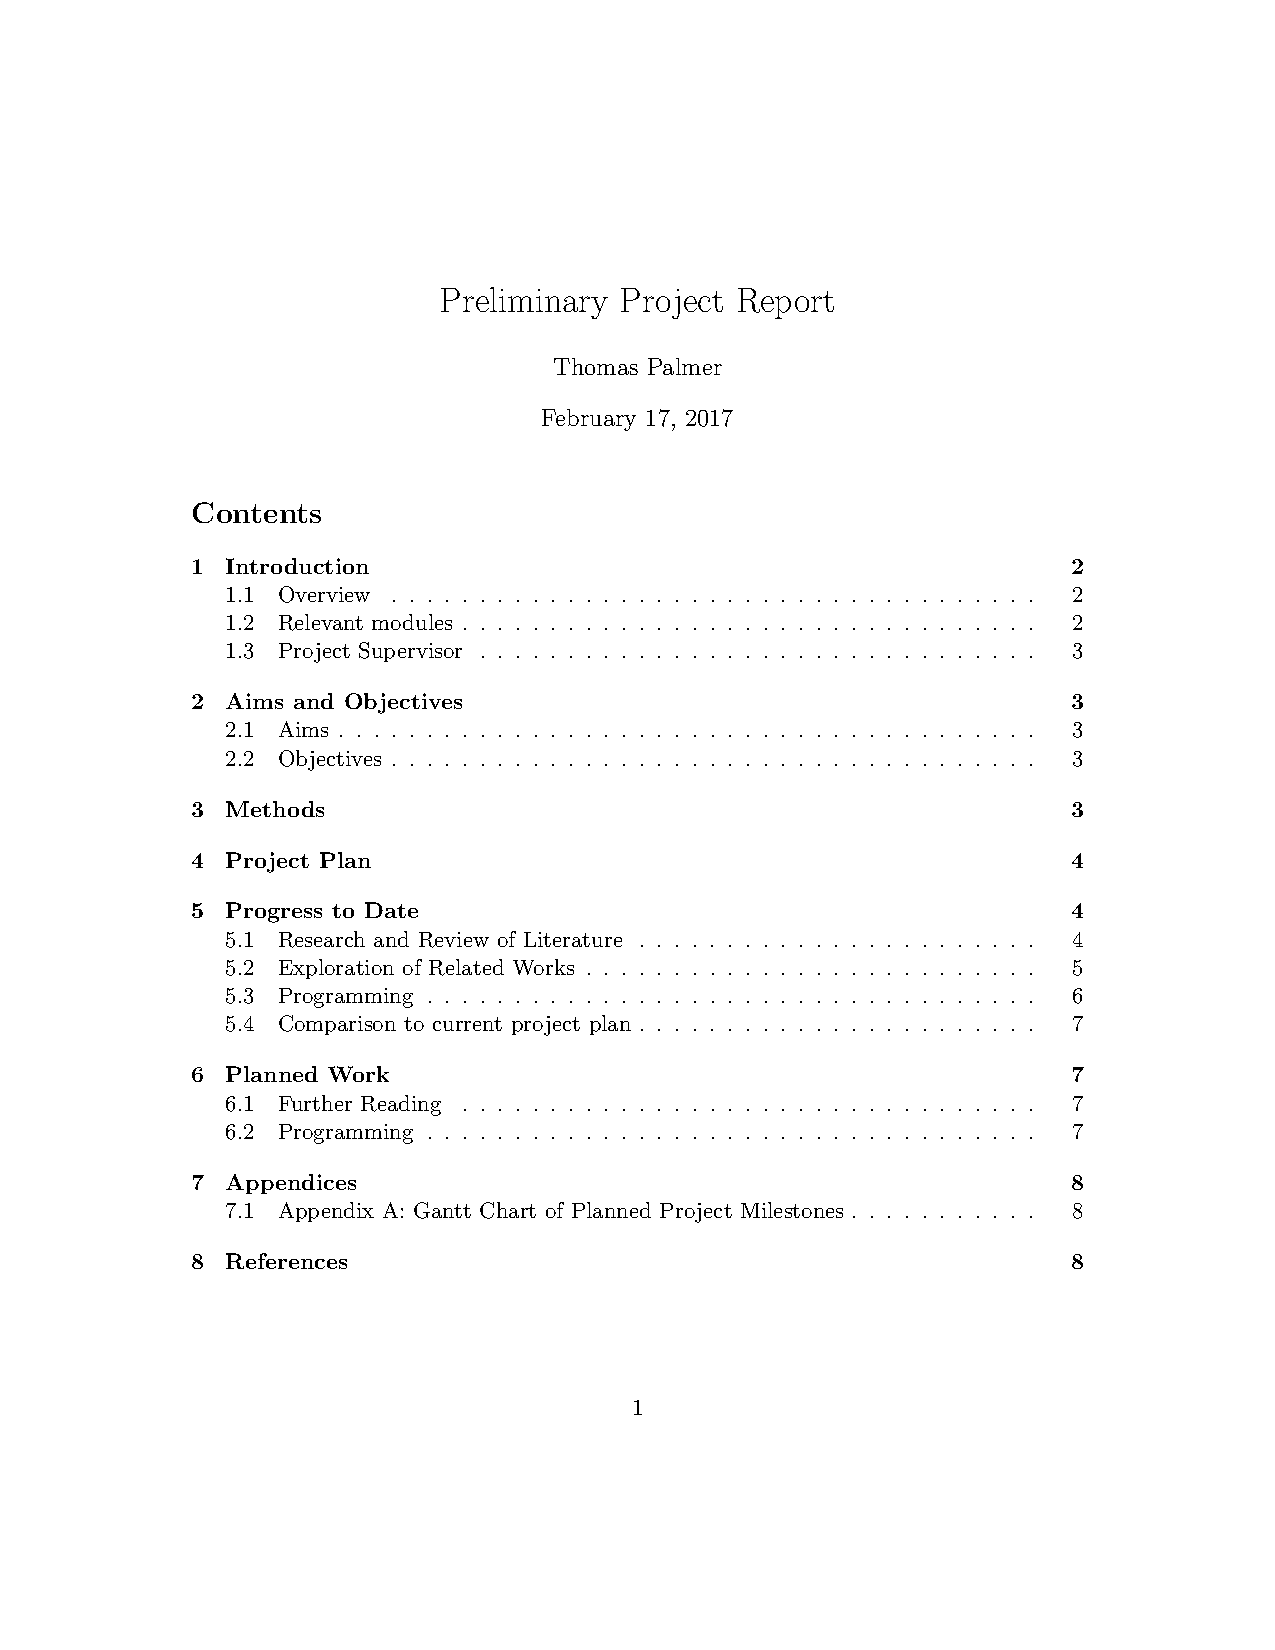
\includepdf[pages={1-},scale=1]{figures/preliminaryReport2}



\section{Project Logs}
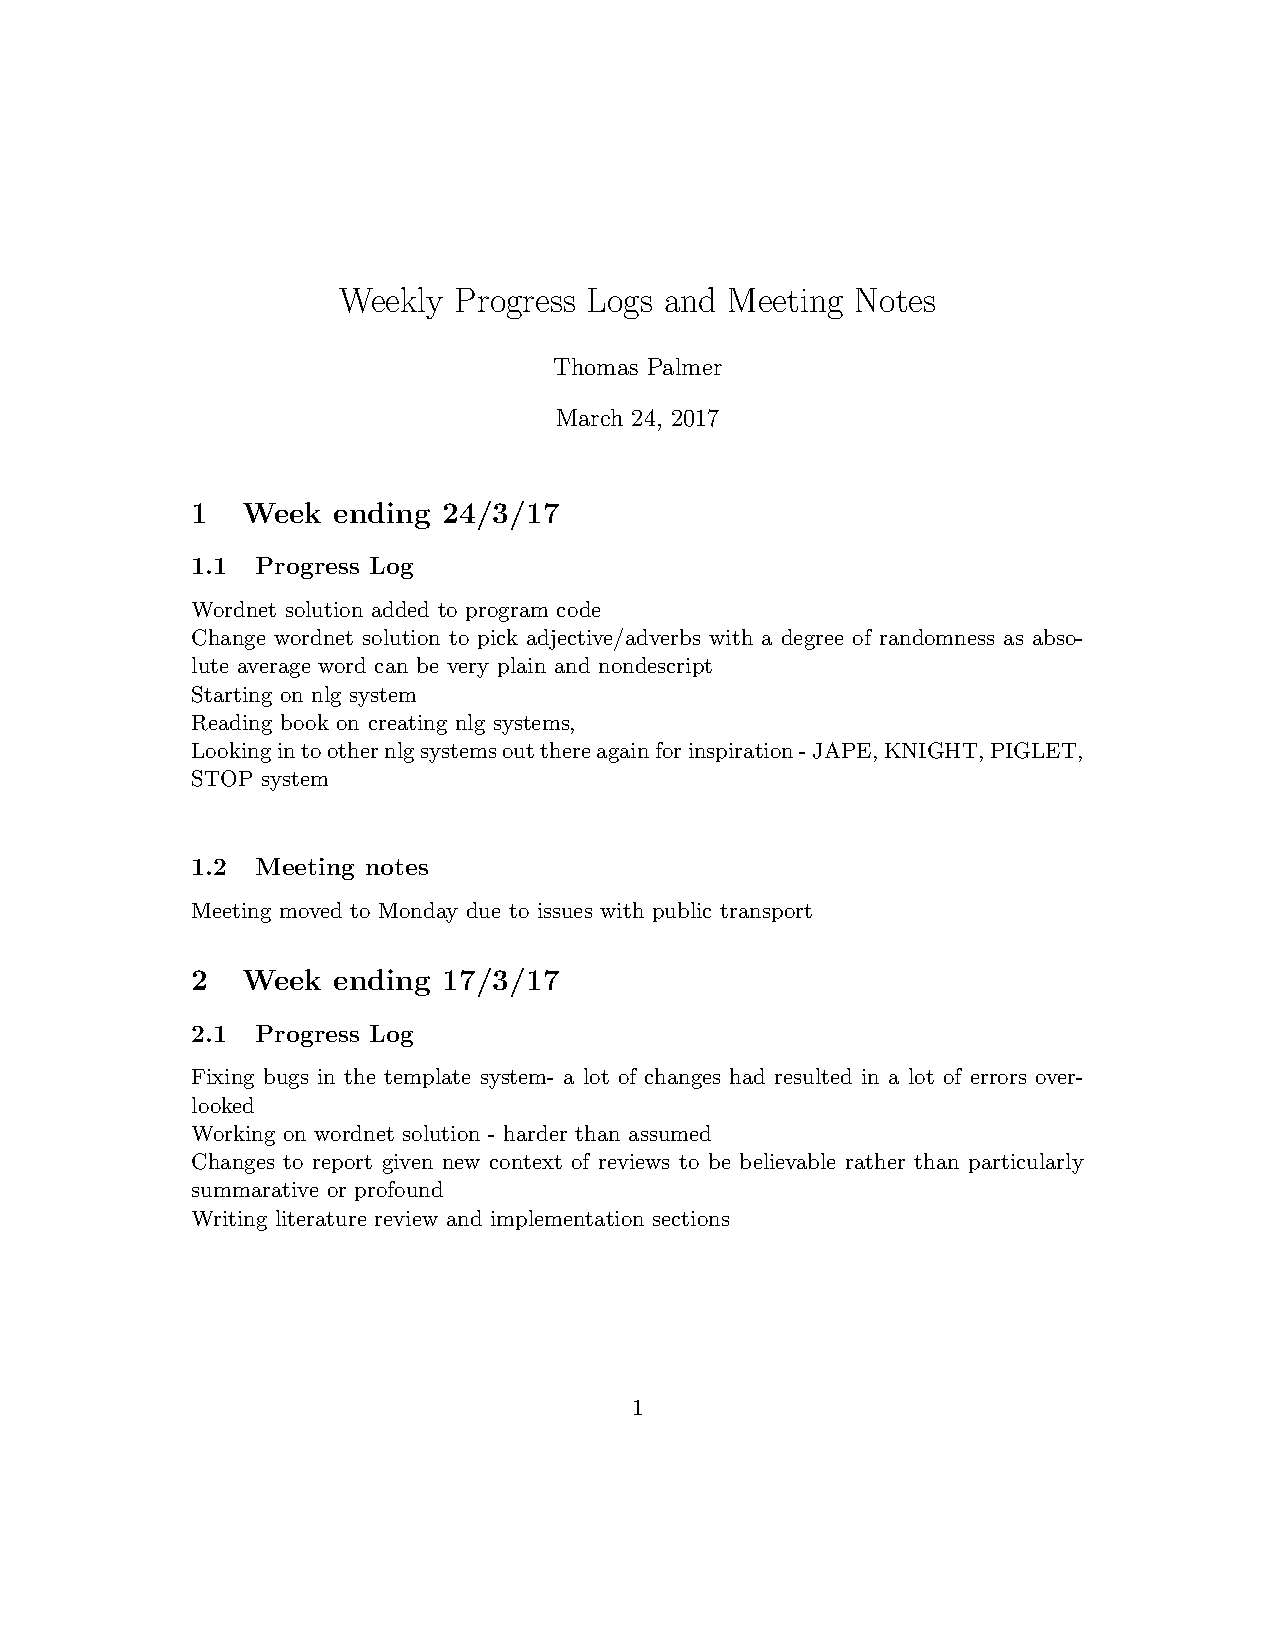
\includepdf[pages={1-}, scale=1]{figures/meetingnotes_17-03-24_thomas-palmer}

\section{Program Code}

\subsection{Python}
\subsection{PHP}
\subsection{mySQL}